\section{Quantum Models}
\label{sec:quantum_models}

The rationale behind building a quantum version of a Game Theory and/or Statistics problem lays in bringing phenomena like quantum superposition, and entanglement into known frameworks allowing different results, that seemingly perform at least as good as their classical versions.

[To Introduce more SOURCES]

The effort put in converting known classical problems also enables the familiarization with the potential differences these models bring.

\subsection{Quantum Roulette}
\label{subsec:quantum_roulette}

In the arbitrary $N$-State quantum roulette,\cite{Salimi2009} presented a $N$-State roulette model using permutation matrices. 

This model is interesting because in captures the usage of permutation matrices to manipulate and change the state of the system.

To verify this model with two players we developed a Matlab simulation \ref{ap:c}, that fellowed the steps taken in \cite{Salimi2009}.

The game in represented in a $N$-Dimensional Hilbert Space. There is a basis in the space that represents each of the equally probable entries as shown in \ref{eq:roulette_1}. In a sense this is a generalization of a quantum coin flip that is also used in Section \ref{sec:quantum_walk_line}.
\begin{equation}
\label{eq:roulette_1}
\vert1\rangle=\left[\begin{array}{c}
1\\
0\\
0\\
\vdots\\
0
\end{array}\right],\:\vert2\rangle=\left[\begin{array}{c}
0\\
1\\
0\\
\vdots\\
0
\end{array}\right],\:\ldots,\:\vert N\rangle=\left[\begin{array}{c}
0\\
0\\
0\\
\vdots\\
1
\end{array}\right]
\end{equation}

Each state transition is obtained using a permutation matrix denoted by $P^{i}$. There are $N!$ permutation matrices, so in the particular case of having a $3$-State roulette, there are $6$ possible transition choices. The classical strategy considered will rely on choosing an arbitrary probability distribution, that verifies\ref{eq:roulette_2}, and that maps the usage of the permutation matrices. This step will not affect the density matrix ($\rho$) of the roulette\ref{eq:roulette_3}.

\begin{equation}
\label{eq:roulette_3}
\rho=\frac{1}{N!}\sum_{i=0}^{N!-1}P^{i}
\end{equation}

\begin{equation}
\label{eq:roulette_2}
\sum_{i=0}^{N!-1}p_{i}=1
\end{equation}

The density matrix is diagonalizable by a Discrete Fourier Transform because it is a kind of circulant matrix\cite{Davis1994}, as we can see in \ref{eq:roulette_4}. In \ref{eq:roulette_4} $\lambda_{k}$ are eigenvalues of $\rho$. $\lambda_{1}=1$
while $\lambda_{2}=\lambda_{3}=\lambda_{k}=\lambda_{N-1}=0$. Each column
$i$ of the Fourier matrix will represent a eigenvector $\vert\lambda_{i}\rangle$.
If we construct the diagonilizing matrix by rotating the columns of
the Fourier Matrix we can obtain the projection states as in \ref{eq:roulette_5}.

\begin{equation}
\label{eq:roulette_4}
F^{\dagger}\rho F=\left[\begin{array}{c}
\lambda_{1}\\
0\\
0\\
\vdots\\
0
\end{array}\begin{array}{c}
0\\
\lambda_{2}\\
0\\
\vdots\\
0
\end{array}\begin{array}{c}
\ldots\\
\ldots\\
\ldots\\
\ddots\\
\ldots
\end{array}\begin{array}{c}
0\\
0\\
0\\
\vdots\\
\lambda_{N-1}
\end{array}\right]
\end{equation}



\begin{equation}
\label{eq:roulette_5}
\vert1\rangle\langle1\vert=\left[\begin{array}{c}
1\\
0\\
0\\
\vdots\\
0
\end{array}\begin{array}{c}
0\\
0\\
0\\
\vdots\\
0
\end{array}\begin{array}{c}
\ldots\\
\ldots\\
\ldots\\
\ddots\\
\ldots
\end{array}\begin{array}{c}
0\\
0\\
0\\
\vdots\\
0
\end{array}\right]=F^{\dagger}\rho F
\end{equation}


The quantum strategy advantage in this case is that the first player
will not alter the density matrix\ref{eq:roulette_6}.

\begin{equation}
\label{eq:roulette_6}
\rho=\sum_{i=0}^{N!-1}p_{i}P^{i}\rho P^{i\dagger},\;\sum_{i=0}^{N!-1}p_{i}=1
\end{equation}

This means that if the second player knows the initial state and the first player plays with a classical strategy, thus never modifing the system density matrix, the second player will be able to manipulade the game under optimal conditions. This result is confirms the demonstration done in \cite{Meyer1999}, on Quantum Strategies, where in a classical $2$ player zero-sum game, if one player adopts a quantum strategy, she increases her chances of winning the game.


\subsection{Prisioner's Dillema}
\label{sebsec:related_work_prisioners_dillama}

The Prisioner's Dillema is one example of a game that can be represented
in normal form\cite{Osborne2004}. This problem has received a great deal of attention
because, in its simple form, rational individuals will seem to deviate
from solutions that would represent the best interest overall solution,
the Pareto Optinal solution. In this game the pareto optimal solution
is not a Nash Equilibrium. The Prisioneers Dillema can be formulated
as it follows:

\begin{quotation}

Two suspects of being partners in a crime are arrested. The police
needs more evidence in order to prossecute the prisioners. So each
prisioner is locked in solitary confinement and has no means of communicating
with the other suspect. The police will then try to extort a confession
from the prisioners. A bargain will be proposed to the suspects:
\begin{itemize}
\item If the suspect testifies against the other suspect (Defects) and the other denies, he will
go free and the second will get three years sentence.
\item If they both testify against one another (both Defect), both will
be convicted and they will get two years.
\item In case both suspects deny the involvement (both Cooperate) of the
other, they will get a one year sentence.
\end{itemize}
\end{quotation}

A matrix representation of the problem is in Table \ref{tab:prisionersdillema_tab1}, a particular case for this problem is represented in Table \ref{tab:prisionersdillema_tab2}. In each cell of the matrix we have a pair of the expected utility for the players for every outcome. A higher utility represents a more desirable state.

In this game the Pareto Optimal solution happens when both players chose to Cooperate (the pair (2,2) in Table \ref{tab:prisionersdillema_tab2}). However both players have the incentive to Defect, because regardless what the opponent choses they will have always a strictly higher payoff. Defecting becomes a dominant strategy in the Prisioner's Dillema and the outcome (Defect, Defect) is a Nash Equilibrium to the game. 

\begin{center}
\begin{table}
\begin{centering}
\begin{tabular}{ccc}
\hline 
 & Player 2: C & Player 2: D\tabularnewline
\hline 
Player 1: C & (R,R) & (S,T)\tabularnewline
Player 1: D & (T,S) & (P,P)\tabularnewline
\hline 
\end{tabular}
\par\end{centering}

\caption{The canonical normal form representation for the Prisioner's Dillema must respect $T>R>P>S$.}
\label{tab:prisionersdillema_tab1}
\end{table}
\par\end{center}

\begin{center}
\begin{table}
\begin{centering}
\begin{tabular}{ccc}
\hline 
 & Player 2: C & Player 2: D\tabularnewline
\hline 
Player 1: C & (2,2) & (0,3)\tabularnewline
Player 1: D & (3,0) & (1,1)\tabularnewline
\hline 
\end{tabular}
\par\end{centering}

\caption{One possible normal form representation of Prisioner's Dillema.}
\label{tab:prisionersdillema_tab2}
\end{table}
\par\end{center}



\subsubsection{Quantum Prisioner's Dillema}
\label{subsubsec:quantum_prisioners_dillema}

The importance of the Prisioner's Dillema for the study of Game Theory made it a prime target for investigation in Quantum Game Theory. The problem has been modelled several times \cite{Eisert2008}\cite{Fra2011a}. Therefore we will use it iin order to exemplify and consolidate the definition described in Section \ref{sec:background_quantum_game_theory}\cite{Fra2011a}. 

Each player $i$ in the quantum version of Prisioner's Dillema will be able to manipulate one qubit ($\varphi_{1}$ and $\varphi_{2}$) in Equations \ref{eq:quantum_prisioner_m1} and \ref{eq:quantum_prisioner_m2}, with two possible operators (shown in Equation \ref{eq:operators_prisioneiros_quanticos}) corresponding to the classical actions: Cooperate (C), and Defect (D). 

\begin{equation}
\label{eq:quantum_prisioner_m1}
\varphi_{1}=a_{0}\vert0\rangle+a_{1}\vert1\rangle,\sum_{i=0}^{1}\vert a_{i}\vert^{2}=1
\end{equation}


\begin{equation}
\label{eq:quantum_prisioner_m2}
\varphi_{2}=b_{0}\vert0\rangle+b_{1}\vert1\rangle,\sum_{j=0}^{1}\vert b_{j}\vert^{2}=1
\end{equation}

\begin{equation}
\label{eq:operators_prisioneiros_quanticos}
\mathcal{U}_{i}=\begin{cases}
O_{i0}=\left[\begin{array}{cc}
1 & 0\\
0 & 1
\end{array}\right]\\
O_{i1}=\left[\begin{array}{cc}
0 & 1\\
1 & 0
\end{array}\right]
\end{cases} , i \in \{ 1, 2 \}
\end{equation}


The system that holds the game is represented in a $\mathcal{H}^{4}$. Each basis ($\vert 1\rangle, \vert 2\rangle, \vert 3\rangle, \vert 4\rangle$), represents a final outcome as Table \ref{tab:prisioners_m} suggests.

\begin{table}
\begin{centering}
\begin{tabular}{ccc}
\hline 
$\bigotimes$ & C-$\vert 0\rangle$ & D-$\vert 1\rangle$\tabularnewline
\hline 
C-$\vert 0\rangle$ & $\vert 0,0\rangle$ & $\vert 0,1\rangle$\tabularnewline
D-$\vert 1\rangle$ & $\vert 1,0\rangle$ & $\vert 1,1\rangle$\tabularnewline
\hline 
\end{tabular}
\par\end{centering}

\caption{Construction of the basis for the game space; $\mathcal{H}^{4}$.}
\label{tab:prisioners_m}
\end{table}



The fundamental difference from the classical version lies in the way the initial state is formulated in Equation \ref{eq:estado_inicial_prisioneiro}. We will entangle our state by applying the gate $\mathcal{J}$ \cite{Letters2002}. The parameter $\gamma$ becomes a way to measure the entanglement in the system\cite{Eisert2008}.

\begin{equation}
\label{eq:matrix_exponencial_esoterica}
\mathcal{J}=exp\left\{ i\frac{\gamma}{2}\left[\begin{array}{cc}
0 & 1\\
1 & 0
\end{array}\right]\otimes\left[\begin{array}{cc}
0 & 1\\
1 & 0
\end{array}\right]\right\}
\end{equation} 

\begin{equation}
\label{eq:estado_inicial_prisioneiro}
%\vert \psi_{in}(\gamma) \rangle= cos( \frac{\gamma}{2})\vert 00\rangle+ isin(\frac{\gamma}{2})\vert 11 \rangle, \gamma \in (0,\pi)
\begin{split}
\vert\psi_{in}(\gamma)\rangle=exp\left\{ i\frac{\gamma}{2}\left[\begin{array}{cc}
0 & 1\\
1 & 0
\end{array}\right]\otimes\left[\begin{array}{cc}
0 & 1\\
1 & 0
\end{array}\right]\right\} \vert00\rangle \\
=cos(\frac{\gamma}{2})\vert00\rangle+isin(\frac{\gamma}{2})\vert11\rangle,\gamma\in(0,\pi)
\end{split}
\end{equation}

\begin{equation}
\vert\psi_{fin}\rangle= \mathcal{J}^{\dagger} \otimes_{i=1}^{2}\mathcal{U}_{i}\vert\psi_{in}\rangle
\label{eq:finalstate_prisioneersdilemma}
\end{equation}

The entanglement in quantum game theory can be viewed as an intrinsic unbreakable contract. Furthermore measuring an entangled state will cause the wave function that describes the state to collapse. Before measuring the final result we will deentangle the system by applying the operator $\mathcal{J}^{\dagger}$, as shown in Equation \ref{eq:finalstate_prisioneersdilemma}.



The utility functions for each player is calculated by projecting the final state in each base and atributing a real number to each measurement, as in equation.
In order to compare a classical version with this quantum model, the real numbers assigned are those in the classical example in Table \ref{tab:prisionersdillema_tab1}, and the basis are presented in Table \ref{tab:prisioners_m}.

\begin{equation}
E_{0}(\vert\psi_{fin}\rangle)=2\times\vert\langle00\vert\psi_{fin}\rangle\vert^{2}+3\times\vert\langle10\vert\psi_{fin}\rangle\vert^{2}+1\times\vert\langle11\vert\psi_{fin}\rangle\vert^{2}
\end{equation}


\begin{equation}
E_{1}(\vert\psi_{fin}\rangle)=2\times\vert\langle00\vert\psi_{fin}\rangle\vert^{2}+3\times\vert\langle01\vert\psi_{fin}\rangle\vert^{2}+1\times\vert\langle11\vert\psi_{fin}\rangle\vert^{2}
\end{equation}

By varying the parameter $\gamma$, we can observe that the expected utility changes as we set up the initial state. Furthermore for $\gamma= \frac{\pi}{4}+k \frac{\pi}{2}, k \in {0, 1, 2, 3}$ the expected utility for each player is $2$ if both players Cooperate, thus removing the dilemma. When the entanglement coeficient is $\gamma= 0+k \frac{\pi}, k \in {0, 1, 2}$ we are left with the classical problem, where there isn't entanglement.

\begin{table}
\begin{center}
\begin{tabular}{cc}
  \num\putindeepbox[7pt]{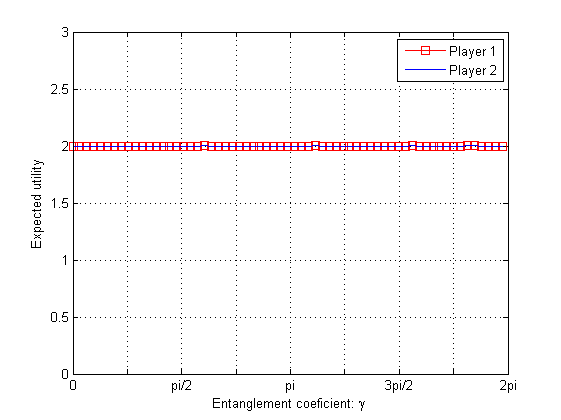
\includegraphics[scale=0.46]{prisionersdillema/II.PNG}}
    & \num\putindeepbox[7pt]{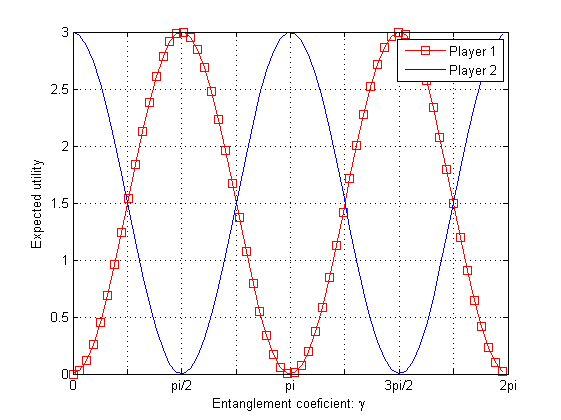
\includegraphics[scale=0.46]{prisionersdillema/InotI.PNG}} \\
  \num\putindeepbox[7pt]{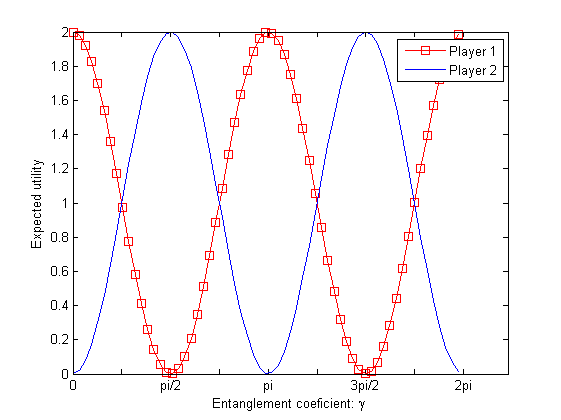
\includegraphics[scale=0.46]{prisionersdillema/notII.PNG}}
    & \num\putindeepbox[7pt]{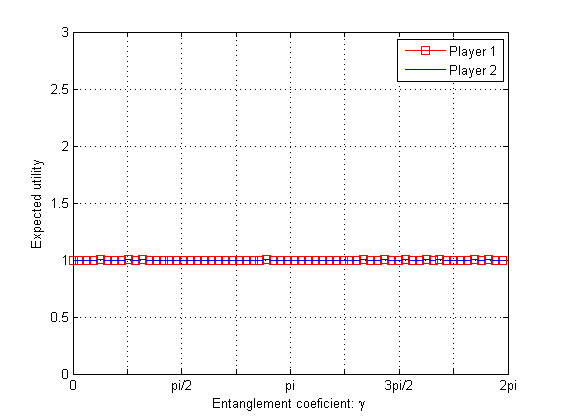
\includegraphics[scale=0.46]{prisionersdillema/notInotI.PNG}} \\
\end{tabular}
\caption{Expected utility for players 1 and 2 giving the entanglement coeficient $\gamma$ used in preparing the inicial state. a) Player 1: Cooperates, Player 2: Cooperates;
b) Player 1: Cooperates, Player 2: Defects; c) Player 1: Defects, Player 2: Cooperates; d) Player 1: Defects, Player 2: Defects. }
\label{tab:prisiones_m_4}
\end{center}
 \end{table}




\subsection{Monty Hall Problem}
\label{subsec:monty_hall}

%%Proffed
The Monty Hall problem became popularized in 1990 in a column, in the magazine Parade\cite{Savant1990}. The reason for its notoriety rests mainly in its counter-intuitive nature. Although the Monty Hall problem can be modeled as a Bayesian probability problem, human beings have difficulty in grasping the probabilities involved.

\subsubsection{Problem Description}
\label{subsubsec:monty_hall_problem description}

The Monty Hall problem is loosely based on a television game show hosted by its namesake - Monty Hall. Furthermore it was first attributed to a statistician, named Selvin. The problem is posed as it follows:
\begin{quotation}
Suppose you're on a game show, and you're given the choice of three doors: Behind one door is a car; behind the others, goats. You pick a door, say No. 1, and the host, who knows what's behind the doors, opens another door, say No. 3, which has a goat. He then says to you, "Do you want to pick door No. 2?" Is it to your advantage to switch your choice?
\end{quotation}

Most people, when faced with this problem, will be indifferent about whether to switch or to stay with the initially picked door.
 
It is also verified that they will tend to stick with their first choice. According to Granberg and Brow\cite{Granberg1995}, only 13\% of 228 subjects decided to switch their initial choice. However, by using probability theory, one can arrive at the conclusion that, in fact, it is advantageous to switch given the previous formulation.
 
The action of the Host implies a belief update on the probabilities of the variables in the system. This poses a violation of rational decision making; subjects do not seem to follow the best strategy which would maximize their chances of winning the prize. 

To understand this exercise, one can look at the decision tree in Figure \ref{fig:monty_hall_tree}. We assumed indifferently that the player chose the door No. 1. The situation is symmetric whichever door she chooses. 

%%Proffed 

Assuming we call $C_{1}$ to the variable that describes whether or not the car in behind door No. 1. The variables $C_{2}$ and $C_{3}$ will respectively describe the probability associated with the car being (or not), behind doors 2 and 3 ($P(C_{2})=1$ or $P(C_{2})=0$, for example).

\begin{figure}[h]
\centering 
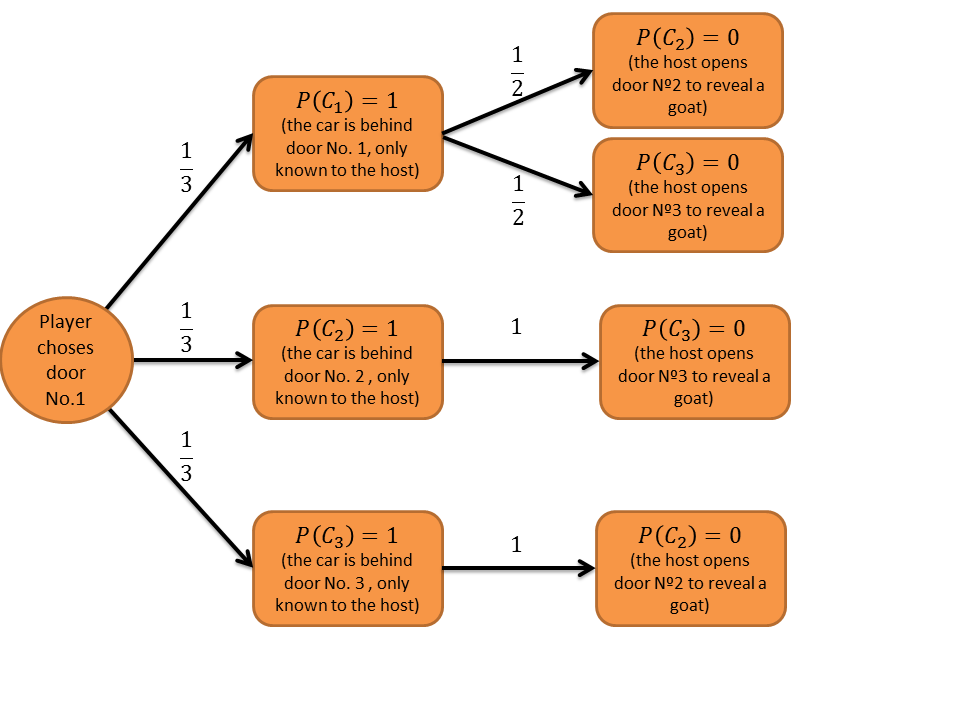
\includegraphics[scale=0.35]{Figures/monty_hall_decision_tree.png}
\caption{Decision tree modelling the Monty Hall problem. }
\label{fig:monty_hall_tree}
\end{figure}

After the player has had her choice, the host will perform an operation on the remaining two doors. The host of the show has complete information of the game, unlike the player.

\begin{equation}
\label{eq:monty_h1}
P(C_{1})=P(C_{1}|\text{\textlnot}C_{2})+P(C_{1}|\text{\textlnot}C_{3})
\end{equation}


\begin{equation}
\label{eq:monty_h2}
P(C_{1})=(\frac{1}{3}\text{\texttimes}\frac{1}{2})+(\frac{1}{3}\text{\texttimes}\frac{1}{2})=1
\end{equation}


\begin{equation}
\label{eq:monty_h3}
P(\text{\textlnot}C_{1})=P(C_{2}|\text{\textlnot}C_{3})+P(C_{3}|\text{\textlnot}C_{2})=(\frac{1}{3}\text{\texttimes}1)+(\frac{1}{3}\text{\texttimes}1)=2/3
\end{equation}

The probability of switching and getting the car is twice \ref{eq:monty_h3} as likely of staying with the first choice and getting the prize\ref{eq:monty_h2}. 


\subsubsection{Quantum Model}

Various Models have been proposed to describe a quantum version of the Monty Hall problem\cite{Gill}\cite{Flitney2008}.

As the host reveals information, the initial setup is modified. This is an interesting property. Despite being a counter-intuitive problem, a quantum approach to this problem allows an in-depth comparison between the classical measurement and the quantum measurement. The classic Monty Hall problem is modeled using conditional probability and Bayes Rule. In the quantum version, measuring the outcome of the final state yields the result, instead of taking into account the intermediate actions \cite{Fra2011}.

Moreover it is important to realize that there is not a unique way to model a classical problem\cite{Gill2002}. Therefore, when modelling a classical problem, we need to select properties that could potentially benefit from a quantum approch. In \cite{Gill2002} we can observe the attempt to stick as closely to the classical formulation as possible, the host has a system that is correlated to the game system.


\section{Overview}
\label{sec:related_work_overview}






